\documentclass[12pt]{article}

\usepackage{fancyhdr} % Required for custom headers
\usepackage{lastpage} % Required to determine the last page for the footer
\usepackage{extramarks} % Required for headers and footers
\usepackage[usenames,dvipsnames]{color} % Required for custom colors
\usepackage{graphicx} % Required to insert images
\usepackage{listings} % Required for insertion of code
\usepackage{courier} % Required for the courier font
\usepackage{lipsum} % Used for inserting dummy 'Lorem ipsum' text into the template
\usepackage{amsmath}
\usepackage{caption}
\usepackage[dvipsnames]{xcolor}

% Margins
\topmargin=-0.45in
\evensidemargin=0in
\oddsidemargin=0in
\textwidth=6.5in
\textheight=9.0in
\headsep=0.25in
\headheight=15.0pt


\linespread{1.1} % Line spacing

% Set up the header and footer
\pagestyle{fancy}
\lhead{\hmwkAuthorName} % Top left header
\chead{\hmwkClass: \hmwkTitle} % Top center head
\cfoot{} % Bottom center footer
\rfoot{Page\ \thepage\ of\ \protect\pageref{LastPage}} % Bottom right footer
\renewcommand\headrulewidth{0.4pt} % Size of the header rule
\renewcommand\footrulewidth{0.4pt} % Size of the footer rule

\setlength\parindent{0pt} % Removes all indentation from paragraphs

%----------------------------------------------------------------------------------------
%	DOCUMENT STRUCTURE COMMANDS
%	Skip this unless you know what you're doing
%----------------------------------------------------------------------------------------

% Header and footer for when a page split occurs within a problem environment
\newcommand{\enterProblemHeader}[1]{
	\nobreak\extramarks{#1}{#1 continued on next page\ldots}\nobreak
	\nobreak\extramarks{#1 (continued)}{#1 continued on next page\ldots}\nobreak
}

% Header and footer for when a page split occurs between problem environments
\newcommand{\exitProblemHeader}[1]{
	\nobreak\extramarks{#1 (continued)}{#1 continued on next page\ldots}\nobreak
	\nobreak\extramarks{#1}{}\nobreak
}

\setcounter{secnumdepth}{0} % Removes default section numbers
\newcounter{homeworkProblemCounter} % Creates a counter to keep track of the number of problems

\newcommand{\homeworkProblemName}{}
\newenvironment{homeworkProblem}[1][Problem \arabic{homeworkProblemCounter}]{ % Makes a new environment called homeworkProblem which takes 1 argument (custom name) but the default is "Problem #"
	\stepcounter{homeworkProblemCounter} % Increase counter for number of problems
	\renewcommand{\homeworkProblemName}{#1} % Assign \homeworkProblemName the name of the problem
	\section{\homeworkProblemName} % Make a section in the document with the custom problem count
	\enterProblemHeader{\homeworkProblemName} % Header and footer within the environment
}{
	\exitProblemHeader{\homeworkProblemName} % Header and footer after the environment
}

\newcommand{\problemAnswer}[1]{ % Defines the problem answer command with the content as the only argument
	\noindent\framebox[\columnwidth][c]{\begin{minipage}{0.98\columnwidth}#1\end{minipage}} % Makes the box around the problem answer and puts the content inside
}

\newcommand{\homeworkSectionName}{}
\newenvironment{homeworkSection}[1]{ % New environment for sections within homework problems, takes 1 argument - the name of the section
	\renewcommand{\homeworkSectionName}{#1} % Assign \homeworkSectionName to the name of the section from the environment argument
	\subsection{\homeworkSectionName} % Make a subsection with the custom name of the subsection
	\enterProblemHeader{\homeworkProblemName\ [\homeworkSectionName]} % Header and footer within the environment
}{
	\enterProblemHeader{\homeworkProblemName} % Header and footer after the environment
}

%----------------------------------------------------------------------------------------
%	NAME AND CLASS SECTION
%----------------------------------------------------------------------------------------

\newcommand{\hmwkTitle}{Assignment\ \#2} % Assignment title
\newcommand{\hmwkClass}{Advanced Image Processing} % Course/class
\newcommand{\hmwkClassInstructor}{Jones} % Teacher/lecturer
\newcommand{\hmwkAuthorName}{Shikhar Vashishth} % Your name
\newcommand{\hmwkAuthorID}{M.Tech CSA - 13374} % Your ID

%----------------------------------------------------------------------------------------
%	TITLE PAGE
%----------------------------------------------------------------------------------------

\title{
	\vspace{2in}
	\textmd{\textbf{\hmwkClass}}\\ 
	\textmd{\textbf{\hmwkTitle}}\\
	\vspace{3in}
}

\author{\textbf{\hmwkAuthorName} \\ {\small \hmwkAuthorID}}
\date{} % Insert date here if you want it to appear below your name

%----------------------------------------------------------------------------------------

\begin{document}
	
\maketitle
\newpage

\begin{homeworkProblem}
\subsection*{Part 1:}


\begin{center}
	\begin{tabular}{||c c c||} 
		\hline
		\textbf{Kernel Size} & \textbf{Standard deviation} & \textbf{Mean Sq. Error} \\ [0.5ex] 
		\hline\hline
		3 & 	 0.10 & 	 99.934713 \\ \hline
		\textbf{3} & 	 \textbf{1.00} & 	 \textbf{89.614492 }\\ \hline
		3 & 	 2.00 & 	 110.292918 \\ \hline
		3 & 	 4.00 & 	 115.660166 \\ \hline
		3 & 	 8.00 & 	 117.003916 \\ \hline
		7 & 	 0.10 & 	 99.934713 \\ \hline
		7 & 	 1.00 & 	 114.808492 \\ \hline
		7 & 	 2.00 & 	 217.848307 \\ \hline
		7 & 	 4.00 & 	 266.146444 \\ \hline
		7 & 	 8.00 & 	 279.693726 \\ \hline
		11 & 	 0.10 & 	 99.934713 \\ \hline
		11 & 	 1.00 & 	 114.857747 \\ \hline
		11 & 	 2.00 & 	 233.674296 \\ \hline
		11 & 	 4.00 & 	 326.976624 \\ \hline
		11 & 	 8.00 & 	 361.110718 \\ \hline
	\end{tabular}
\end{center}

The best low pass Gaussian filter was of \textbf{size 3} with \textbf{standard deviation 1.0}. 

\paragraph{Observations:}
\begin{enumerate}
\item
From the observed MSE values we can see that as we increase the size of the Gaussian filter and the value of the standard deviation, the blurness in the image increases which in turn increases the MSE error.
\item
The mean square error with sigma = .1 remains almost the same for all the kernel sizes because, the kernels generated in all these cases have middle entry as 1 and all other entries are of order $\approx 10^{-40}$ which give us back the same noisy image. That is the reason why Gaussian filters with low variance (0.1) are not optimal. On the other hand, if we increase the size of the filter and its variance too much then the resulting image becomes too blurred and thus, more away from the desired image. Therefore, a filter with moderate size and variance gave us the best results.

\begin{figure}[h]
	\centering
	\fbox{\includegraphics[width=16cm]{../q1_1/comp.jpg}}
	\caption{Choosing optimal low pass Gaussian filter}
\end{figure}

\end{enumerate}
\clearpage

\subsection{Part 2:}
Variance of high pass of the original image $y_1$:
$$ \sigma_{y_1}^2 = \frac{1}{MN}\sum_{j=1}^{N}\sum_{i=1}^{M}y_1^2(i,j) = 148.1371$$

Variance of noise in the high pass image $z_1$:
$$ \sigma_{z_1}^2 = (1-w(0,0))^2\sigma_{z_1}^2 + \sum_{l,k [(l,k) \ne (0,0)]}(w(k,l))^2  \sigma_{z_1}^2= 71.7244$$

\begin{figure}[h]
	\centering
	\fbox{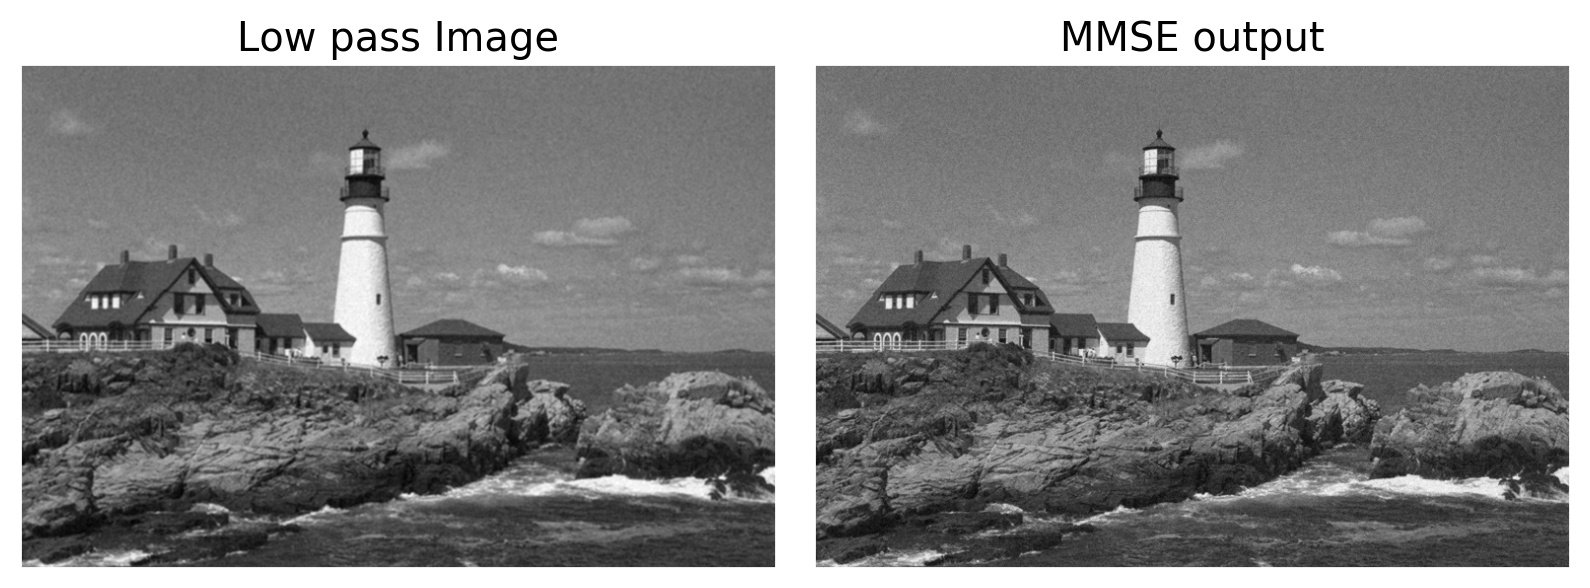
\includegraphics[width=16cm]{../mmse.jpg}}
\end{figure}

\begin{figure}[h]
	\centering
	\fbox{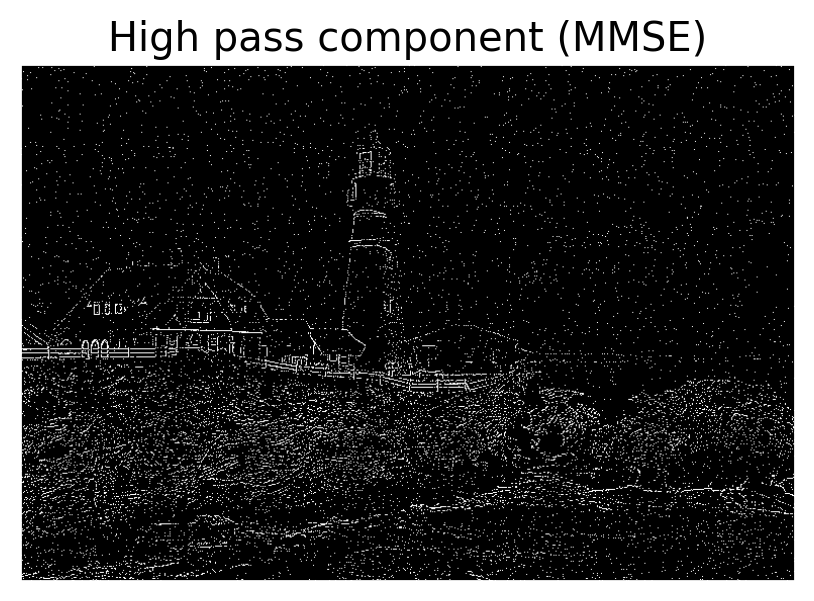
\includegraphics[width=8cm]{../mmse_hp.png}}
	\caption{Applying MMSE filter}
\end{figure}

The value of MSE of low pass component obtained after applying gaussian filter was \textbf{89.6144 }and after applying MMSE filter ($\hat{x} = \mu_y + \hat{x_1}$)the value of MSE reduced to \textbf{57.9407}.

\clearpage
\paragraph*{Observations:}
\begin{enumerate}
	\item
	We can clearly see that the mean squared error has reduced on adding the high frequency component, $\hat{x_1}$ to the low pass component, $\mu_y$. Thus MMSE has made the output more closer to the original image. 
	\item
	Although the low pass output of the gaussian filter and MMSE output are visually not easily differentiable but on careful analysis one can see that MMSE output is more sharper than the low pass image.
	\item
	The figure 2 shows the high pass component of the image which was getting thrown away with the noise. It helps us understand why the MMSE method is able to give us better results.
\end{enumerate}

%------------------------------------------------------------------------------
\clearpage
\subsection*{Part 3: SureShrink}
\begin{figure}[h]
	\centering
	\fbox{\includegraphics[width=14cm]{../q1_1/3_sureComp}}
	\caption{Comparing SURE for different values of 't'}
\end{figure}

The minimum value of SURE is obtained at threshold(t) = \textbf{9.2964}.

\begin{table}[h]
	\begin{center}
		\begin{tabular}{||c c ||} 
			\hline 
			\textbf{Threshold (t)} & \textbf{MSE} \\ [0.5ex] 
			\hline \hline
			7.45 &	51.9138 \\ \hline
			7.98 &	50.9634 \\ \hline
			8.51 &	50.2244 \\ \hline
			9.03 &	49.6786 \\ \hline
			\textbf{9.30} (\textit{SureShrink})&	\textbf{49.4724} \\ \hline
			10.09 &	49.0986 \\ \hline
			\textbf{10.61} (\textit{Best}) &	\textbf{49.0355} \\ \hline
			11.14 &	49.1028 \\ \hline
			11.66 &	49.2875 \\ \hline
			12.72 &	49.9651 \\ \hline
		\end{tabular}
		\caption{MSE of shrinkage estimator for different thresholds}
	\end{center}
\end{table}

\clearpage
\begin{figure}[h]
	\centering
	\fbox{\includegraphics[width=16cm]{../q1_1/3_shrink_comp}}
	\caption{Comparing Shrink Estimator output with low pass output}
\end{figure}

MSE for Shrinkage estimator: \textbf{49.4724} \\
MSE for MMSE output: \textbf{57.9407} \\
MSE for Low pass Image: \textbf{89.6144}

\paragraph{Observations:}
\begin{enumerate}
	\item 
	The SURE value attains minimum at threshold = 9.2964 and start rising and become constant after threshold = 80.
	\item
	The Table 1  verifies the optimality of the threshold given by \textit{SureShrink} method. We can see that although the best value of threshold (with minimum MSE) is around 10.61 but \textit{SureShrink} gives us threshold value as 9.2964 which is quite close to the optimum value.
	\item
	Using the threshold, obtained from SureShrink method, in Shrink Estimator gives us a considerable decrease in MSE. This method gives us better results as compared to MMSE method and gaussian low pass filter.
\end{enumerate}

\clearpage
\subsection*{Part 4: Two scale SureShrink}


\subsubsection{Selecting Gaussian kernel for second scale}
\begin{table}[h]
\begin{center}
	\begin{tabular}{||c c c||} 
		\hline
		\textbf{Kernel Size} & \textbf{Standard deviation} & \textbf{Mean Sq. Error} \\ [0.5ex] 
		\hline\hline
		\textbf{17} & 	 \textbf{8.00} &  	 \textbf{442.986165} \\ \hline
		17 & 	 12.00 &  	 460.042155 \\ \hline
		17 & 	 16.00 &  	 466.232666 \\ \hline
		21 & 	 8.00 &  	 478.722046 \\ \hline
		21 & 	 12.00 &  	 506.104411 \\ \hline
		21 & 	 16.00 &  	 516.328451 \\ \hline
		23 & 	 8.00 &  	 493.173014 \\ \hline
		23 & 	 12.00 &  	 526.761759 \\ \hline
		23 & 	 16.00 &  	 539.532837 \\ \hline
		25 & 	 8.00 &  	 505.500814 \\ \hline
		25 & 	 12.00 &  	 545.830444 \\ \hline
		25 & 	 16.00 &  	 561.479736 \\ \hline
		31 & 	 8.00 &  	 531.173462 \\ \hline
		31 & 	 12.00 &  	 593.426188 \\ \hline
		31 & 	 16.00 &  	 619.436320 \\ \hline
	\end{tabular}
	\caption{Selecting Gaussian kernel for second scale}
\end{center}
\end{table}
The best (lowest MSE) Gaussian filter for second scale was of \textbf{size 17} with \textbf{standard deviation 8.0}.

\subsubsection{Choosing suitable threshold for Shrinkage estimator}
Estimating variance of low pass noise ($\sigma_{\mu_Z}^2 $)
$$ \sigma_{\mu_Z}^2 = \sum_{k}^{} \sum_{l}^{} w_1(k,l)^2 \sigma_Z^2 = 12.5604$$

Estimating variance of noise of high pass in low pass of the image ($\sigma_{Z_2}^2$)
$$ \sigma_{Z_2}^2 = (1-w_2(0,0))^2\sigma_{\mu_Z}^2 + \sum_{l,k [(l,k) \ne (0,0)]}(w_2(k,l))^2  \sigma_{\mu_Z}^2= 12.4829$$

\begin{figure}[h]
	\centering
	\fbox{\includegraphics[width=12cm]{../q1_1/4_sureComp}}
	\caption{Comparing SURE for different values of 't'}
\end{figure}

\begin{figure}[h]
	\centering
	\fbox{\includegraphics[width=16cm]{../q1_1/4_shrink_comp}}
	\caption{Comparing SURE for different values of 't'}
\end{figure}

\clearpage
\textbf{Comparing MSE:} \\
Two scale based on Shrinkage Estimator: \textbf{49.1538} \\
One scale based on Shrinkage Estimator: \textbf{49.4724} \\
MMSE method: \textbf{57.9407} \\
Gaussian low pass filter: \textbf{89.6144}

\paragraph{Observations:}
\begin{enumerate}
	\item
	From the above results, we can easily see that the two scale denoising based on \textit{SureShrink} has further improved the quality of results. The MSE of the final output has further reduced which shows that it has become more closer to the original desired image. Moreover, the bottom right image in the above figure shows the high pass information in the low pass of the image which was not getting utilized by the other approaches discussed before.
	\item
	For the second phase a different low pass filter was used because reusing the same filter from the first phase will not lead to any change in the low pass image. The following results proves this observation. On applying the same filter the MSE of new low pass image obtained got changed by only \textbf{11.1581}. But if we apply Gaussian filter of larger size and sigma value then the change in MSE is significant. Change in MSE with Gaussian of size 17 and sigma 4 was \textbf{200.2483} and with size 31 and sigma 8 was \textbf{358.5539.} 
	\begin{figure}[h]
		\centering
		\fbox{\includegraphics[width=12cm]{../q1_1/same_filter}}
		\caption{Consequences of using same filter in second pass}
	\end{figure}

\end{enumerate}

\end{homeworkProblem}

%**********************************************************************************
\clearpage
\begin{homeworkProblem}
\begin{figure}[h]
	\centering
	\fbox{\includegraphics[width=8cm]{../q2/hp_comp}}
	\caption{High pass component obtained using given filter}
\end{figure}

\subsection{Part 1: Constant Gain}

\begin{figure}[h]
	\centering
	\fbox{\includegraphics[width=8cm]{../q2/mse_gain_comp}}
	\caption{MSE vs gain}
\end{figure}

\begin{figure}[h]
	\centering
	\fbox{\includegraphics[width=16cm]{../q2/lp_gain_comp}}
	\caption{Comparing low pass and sharpened image}
\end{figure}

\clearpage
\subsubsection{Observations:} 
\paragraph{}
We can clearly see from the graph between MSE and gain that as the gain increases the MSE also increases. This is because 
$$\hat{x} = \mu_y + \lambda y_1 \text{, where $y_1$ is high pass component of the image}$$ 

\quad Since, the high component of the image also contains noise other than the edge information therefore, as we amplify high pass component the noise in the image also gets amplified which we can clearly see from the bottom right image in the above figure. Moreover, because the Laplacian filter was used for getting the high pass component, along with the edge information the noise also got captured. We can see from the graph that the MSE error becomes linear function of gain for its large values.
\clearpage
\subsection{Part 2: Variable Gain}
\begin{figure}[h]
	\centering
	\includegraphics[width=14cm]{../q2/3dplot}
	\caption{Getting optimal values of m and t}
\end{figure}

The lowest MSE was obtained at \textbf{m = 0.002 }and \textbf{t = 89.0}. \\

\textbf{Comparing MSE:} \\
Low Pass Filter: \textbf{89.6383} \\
Constant Gain: \textbf{68.6534} \\
Variable Gain: \textbf{63.3468} 

\begin{figure}[h]
	\centering
	\includegraphics[width=8cm]{../q2/gain_func}
	\caption{Gain variation vs y1 for chosen (m,t)}
\end{figure}


\begin{figure}[h]
	\centering
	\fbox{\includegraphics[width=16cm]{../q2/var_gain}}
	\caption{Visual output with variable gain}
\end{figure}

\clearpage
\paragraph{Observations}
\begin{enumerate}
	\item As compared to constant gain, the variable gain gave us better results in terms of MSE and visually as well. 
	\item The optimum value of constant gain gave us the range to search for the optimum values of parameters $m$ and $t$. As the search range of $m$ and $t$ has to be such that $m \times t$ should be near to the optimal constant gain value for atleast one combination. In the above setup I chose a large value ($0,100$) for $t$ because the gain is defined as:
	\[ 
		\lambda(y_1) =
		\begin{cases} 
			m|y_1| & |y_1| \leq t \\
			mt & o.w. 
		\end{cases}
	\]
	So, for any small value of t will make the variable gain will be almost constant as it will affect only a small range of $y_1$. And for keeping the product of $m$ and $t$ near to the optimal of constant gain I chose $m$ range to be small ($.001, .004$)
	
	\begin{figure}[h]
		\centering
		\fbox{\includegraphics[width=12cm]{../q2/mt_gain}}
		\caption{Visual comparison for different (m,t) combinations}
	\end{figure}
	
	\textbf{MSEs: 15098.0013, 89.6205, 69.6400, 68.8058} respectively
	
	We can see from the above results that if we take large values for both $m$ and $t$ then we get completely spoiled result. On using small values for both $m$ and $t$ we get no improvement in the MSE from low pass image. But one using values of $m$ and $t$ such that their product is approximately equal to the optimal value obtained in case of constant gain we experience much better results which proves the correctness of our observation.	
\end{enumerate}

\end{homeworkProblem}

\end{document}